% Compilar con pdfLaTeX
% Este documento usa newtxtext y newtxmath como aproximación a Times New Roman
% Para Times New Roman exacto, usar XeLaTeX/LuaLaTeX con fontspec

% ======================== REGLAS DEL TEMPLATE ========================
% - Español
% - Paper universitario clásico
% - 11 pt
% - Times New Roman o equivalente
% - Bloque inicial centrado en una columna
% - Resumen a ancho completo
% - Cuerpo en dos columnas
% - Encabezado con línea fina
% - Pie con número centrado
% - Secciones en romanos mayúsculos
% - Subsecciones I.1
% - Subsubsecciones I.3.1
% - Estilo sobrio y académico

% ======================== REGLAS PARA FIGURAS, GRÁFICOS Y TABLAS ========================
% - Todas las figuras, gráficos y tablas deben usar captions consistentes definidos GLOBALMENTE (no manual por cada caso)
% - Formato del caption:
%     "Figura 1. Descripción..."
%     "Tabla 1. Descripción..."
%     "Gráfico 1. Descripción..." (si aplica)
% - Debe haber un PUNTO después del número (ej: "Figura 1.")
% - El caption debe ir:
%     - DEBAJO en figuras y gráficos
%     - (preferiblemente) DEBAJO en tablas para mantener consistencia
% - El caption debe estar CENTRADO
% - El caption debe estar en CURSIVA
% - Tamaño de fuente ligeramente menor o igual al texto principal
% - Espaciado compacto (estilo paper)
% - No usar estilos modernos ni decorativos
% - No usar colores (mantener estilo académico clásico)
% - La etiqueta (Figura, Tabla, etc.) y el texto deben seguir el mismo estilo visual
% - Debe haber separación adecuada entre la figura/tabla y el caption
% - Los captions no deben romper el flujo en dos columnas

% ======================== CONTROL DE FLOTANTES ========================
% - Figuras y tablas deben respetar el formato en dos columnas
% - Evitar que los flotantes desordenen el documento
% - Usar posicionamiento adecuado (htbp o similar)
% - Mantener consistencia en todo el documento

\documentclass[11pt,letterpaper]{article}

% ======================== PAQUETES ========================
\usepackage[spanish]{babel}
\usepackage[utf8]{inputenc}
\usepackage[T1]{fontenc}

% Renombrar Figura a Gráfico y Cuadro a Tabla (debe ir después de babel)
\addto\captionsspanish{
    \renewcommand{\figurename}{Gráfico}
    \renewcommand{\tablename}{Tabla}
}

% Tipografía Times New Roman (aproximación con pdfLaTeX)
\usepackage{newtxtext,newtxmath}

% Geometría - márgenes estrechos tipo paper
\usepackage[
    top=2cm,
    bottom=2.5cm,
    left=1.8cm,
    right=1.8cm,
    headheight=14pt,
    headsep=0.4cm,
    footskip=1cm
]{geometry}

% Encabezados y pies de página
\usepackage{fancyhdr}
\pagestyle{fancy}
\fancyhf{}
\fancyhead[L]{\small Laboratorio de Física I}
\fancyhead[R]{\small Exp 1: Caída Libre}
\fancyfoot[C]{\thepage}
\renewcommand{\headrulewidth}{0.4pt}
\renewcommand{\footrulewidth}{0.4pt}

% Dos columnas
\usepackage{multicol}
\setlength{\columnsep}{0.6cm}

% Figuras y tablas
\usepackage{graphicx}
\usepackage{float}
\usepackage{caption}

% Configuración global de captions según las reglas del template
\captionsetup{
    format=plain,              % Formato simple
    labelsep=period,          % PUNTO después del número (ej: "Tabla 1.")
    justification=centering,  % CENTRADO
    font={small,it},          % Tamaño pequeño y CURSIVA (itálica)
    labelfont={small,it,bf},  % Etiqueta: pequeña, cursiva y negrita
    position=bottom,          % Caption DEBAJO (tanto figuras como tablas)
    skip=4pt,                 % Separación entre figura/tabla y caption (más reducido)
    aboveskip=4pt,           % Espacio adicional arriba del caption (más reducido)
    belowskip=6pt            % Espacio después del caption (consistente)
}

% Asegurar que tablas también tengan caption debajo
\captionsetup[table]{position=bottom}
\captionsetup[figure]{position=bottom}

% Tablas
\usepackage{array}
\usepackage{booktabs}

% Matemáticas
\usepackage{amsmath}
\usepackage{amssymb}

% Interlineado compacto
\usepackage{setspace}
\setstretch{1.0}

% Espaciado de párrafos
\setlength{\parindent}{0.5cm}
\setlength{\parskip}{0pt}

% Personalización de títulos de sección
\usepackage{titlesec}

% Secciones principales: números romanos en mayúscula, alineadas a la izquierda
\titleformat{\section}
    {\normalfont\fontsize{11}{13}\bfseries}
    {\Roman{section}.}
    {0.5em}
    {\MakeUppercase}

\titlespacing*{\section}
    {0pt}{9pt plus 1pt minus 1pt}{5pt plus 1pt minus 1pt}

% Subsecciones: numeración tipo I.1
\titleformat{\subsection}
    {\normalfont\fontsize{11}{13}\bfseries}
    {\Roman{section}.\arabic{subsection}}
    {0.5em}
    {}

\titlespacing*{\subsection}
    {0pt}{7pt plus 1pt minus 1pt}{4pt plus 1pt minus 1pt}

% Subsubsecciones: numeración tipo I.1.2 (sin punto final)
\titleformat{\subsubsection}
    {\normalfont\fontsize{11}{13}\bfseries}
    {\Roman{section}.\arabic{subsection}.\arabic{subsubsection}}
    {0.5em}
    {}

\titlespacing*{\subsubsection}
    {0pt}{6pt plus 1pt minus 1pt}{4pt plus 1pt minus 1pt}

% Ajustes para listas
\usepackage{enumitem}
\setlist{noitemsep,topsep=3pt,parsep=0pt,partopsep=0pt}

% Control adicional de espaciado en flotantes
\setlength{\floatsep}{4pt plus 1pt minus 1pt}        % Espacio entre flotantes consecutivos (reducido)
\setlength{\textfloatsep}{6pt plus 1pt minus 1pt}   % Espacio entre flotante y texto (reducido)
\setlength{\intextsep}{4pt plus 1pt minus 1pt}      % Espacio alrededor de flotantes en el texto (reducido)

% ======================== INICIO DEL DOCUMENTO ========================
\begin{document}

% Desactivar encabezado y pie en la primera página
\thispagestyle{empty}

% ======================== BLOQUE INICIAL (UNA COLUMNA) ========================

\begin{center}
    {\fontsize{14}{16}\selectfont\bfseries 
    Determinación experimental de la aceleración de gravedad mediante caída libre}
    
    \vspace{0.3cm}
    
    {\normalsize
    Adriana Elisa Aylas Dominguez, Maximiliano Renato Ossandón Fuentealba,\\
    Rafael Ignacio Arechavala Huenchual}
    
    \vspace{0.2cm}
    
    {\small\itshape
    Instituto de Física, Pontificia Universidad Católica de Chile, Santiago 7820436, Chile}
    
    \vspace{0.2cm}
    
    {\small 20 de abril de 2026}
\end{center}

\vspace{0.3cm}

% Resumen en una columna
\noindent\textbf{Resumen.} En este laboratorio se buscó determinar experimentalmente la aceleración de la gravedad analizando la caída de un objeto desde distintas alturas. Para ello, se midieron varias veces los tiempos de caída con el fin de obtener datos más confiables y, posteriormente, se realizaron cálculos para estimar un valor aproximado de la gravedad.
Además, se utilizó una fotocelda para estudiar con mayor precisión el movimiento durante la caída, lo que permitió analizar cómo varía la velocidad en función del tiempo. A partir de ambos métodos, se compararon los resultados obtenidos y se observó que no siempre se alcanzan valores exactos, principalmente debido a errores de medición.
En términos generales, la experiencia permitió comprender mejor el fenómeno de la caída libre y reconocer la importancia de realizar mediciones cuidadosas y de analizar adecuadamente los datos experimentales.

\vspace{0.2cm}

\noindent\textbf{Palabras clave:} caída libre, aceleración de gravedad, movimiento uniformemente acelerado, fotocelda, errores experimentales.

\vspace{0.4cm}

% ======================== INICIO DE DOS COLUMNAS ========================
\begin{multicols}{2}
\raggedcolumns  % Evita estiramiento vertical en columnas (mejor que raggedbottom para multicols)

% ======================== I. INTRODUCCIÓN ========================
\section{Introducción}

En física, la caída libre es un tipo de movimiento en el cual un objeto se desplaza únicamente bajo la acción de la gravedad. Este fenómeno es importante porque permite estudiar una de las constantes fundamentales de la naturaleza: la aceleración de la gravedad.

En este laboratorio, el objetivo fue determinar experimentalmente el valor de esta aceleración utilizando mediciones de tiempo y altura. Para ello, se aplicaron distintos métodos, como el uso de cronómetro y fotocelda, con el propósito de comparar resultados y comprender mejor las posibles fuentes de error presentes en la experiencia.

Este experimento permite relacionar conceptos teóricos con la práctica y, además, desarrollar habilidades en la toma de datos, el tratamiento de resultados y el análisis experimental.

% ======================== I.1 Objetivos ========================
\subsection{Objetivos}

Determinar experimentalmente la aceleración de la gravedad mediante dos métodos distintos: medición manual de tiempo de caída y registro automático con fotocelda.

Comparar los resultados obtenidos mediante ambos procedimientos, analizando la precisión y confiabilidad de cada método.

Aplicar herramientas estadísticas para cuantificar la dispersión de los datos y la incertidumbre asociada al valor experimental de la gravedad.

% ======================== I.2 Hipótesis ========================
\subsection{Hipótesis}

Si se mide el tiempo que tarda un objeto en caer desde distintas alturas, entonces será posible calcular un valor cercano a la aceleración de la gravedad, ya que el movimiento de caída libre depende directamente de esta magnitud. Sin embargo, es esperable que el resultado no sea exacto debido a errores asociados a la medición del tiempo, la altura y otras condiciones experimentales.

% ======================== I.3 Marco teórico ========================
\subsection{Marco teórico}

La caída libre corresponde al movimiento de un objeto sometido únicamente a la acción de la gravedad, despreciando la resistencia del aire. En este tipo de movimiento, la aceleración es constante y corresponde a la aceleración de gravedad, denotada por $g$.

Cuando un objeto se deja caer desde el reposo, su movimiento puede describirse mediante la ecuación del movimiento rectilíneo uniformemente acelerado:
\begin{equation}
h_f = h_i + v_i t - \frac{1}{2}gt^2
\end{equation}

donde $h_f$ es la posición final, $h_i$ la posición inicial, $v_i$ la velocidad inicial, $t$ el tiempo transcurrido y $g$ la aceleración de gravedad.

Para este experimento, el objeto se suelta desde el reposo, por lo que $v_i=0$, y se considera que llega al suelo, es decir, $h_f=0$. Entonces, la ecuación se simplifica a:
\begin{equation}
0 = h_i - \frac{1}{2}gt^2
\end{equation}

De esta expresión se obtiene:
\begin{equation}
h_i = \frac{1}{2}gt^2
\end{equation}

y despejando la gravedad:
\begin{equation}
g = \frac{2h_i}{t^2}
\end{equation}

Esta fórmula se utiliza en el primer procedimiento para calcular la aceleración de gravedad a partir de la altura y del tiempo de caída medido.

Por otra parte, en el segundo procedimiento se emplea una fotocelda, la cual permite registrar intervalos de tiempo durante la caída de una regleta. A partir de estos datos, se calcula la velocidad media en cada tramo mediante:
\begin{equation}
v = \frac{\Delta x}{\Delta t}
\end{equation}

donde $\Delta x$ es la distancia recorrida en cada intervalo y $\Delta t$ el tiempo correspondiente.

Además, el tiempo asociado a cada velocidad se obtiene usando el tiempo promedio entre dos registros consecutivos:
\begin{equation}
t_{\text{prom}} = \frac{t_i + t_{i+1}}{2}
\end{equation}

Con estos valores, se construye un gráfico de velocidad en función del tiempo. Si el movimiento es uniformemente acelerado, se espera obtener una relación lineal de la forma:
\begin{equation}
v(t)=gt+b
\end{equation}

donde la pendiente de la recta corresponde a la aceleración de gravedad experimental.

Como en la práctica siempre existen errores en la medición, es necesario repetir varias veces el experimento y analizar estadísticamente los resultados. Para ello, se utiliza la media aritmética:
\begin{equation}
\bar{x}=\frac{1}{n}\sum_{i=1}^{n}x_i
\end{equation}

la desviación estándar muestral:
\begin{equation}
s=\sqrt{\frac{1}{n-1}\sum_{i=1}^{n}(x_i-\bar{x})^2}
\end{equation}

y el error estándar de la media:
\begin{equation}
d_x=\frac{s}{\sqrt{n}}
\end{equation}

Estas expresiones permiten obtener un valor representativo, cuantificar la dispersión de los datos y estimar la incertidumbre asociada al resultado experimental.

% ======================== II. MONTAJE Y PROCEDIMIENTO EXPERIMENTAL ========================
\section{Montaje y procedimiento experimental}

% ======================== II.1 Montaje ========================
\subsection{Montaje}

En este laboratorio se determinó experimentalmente la aceleración de la gravedad midiendo el tiempo de caída de un objeto desde distintas alturas. Para ello, se marcaron tres alturas y se dejó caer el objeto desde el reposo, registrando el tiempo con un cronómetro. Cada medición se repitió varias veces con el fin de reducir errores experimentales.

Con los datos obtenidos, se calculó la aceleración de la gravedad para cada caso y posteriormente se promediaron los resultados.

En una segunda parte, se utilizó una fotocelda para registrar intervalos de tiempo durante la caída de una regleta. A partir de estos datos, se calcularon velocidades y se construyó un gráfico de velocidad en función del tiempo, cuya pendiente permitió obtener una estimación experimental de la aceleración de la gravedad.

Finalmente, se compararon los resultados obtenidos con ambos métodos y se analizaron las posibles fuentes de error presentes en la experiencia.

% ======================== III. RESULTADOS ========================
\section{Resultados}

% ======================== III.1 Procedimiento 1 ========================
\subsection{Procedimiento 1}

% ======================== III.1.1 Datos obtenidos ========================
\subsubsection{Datos obtenidos}

\begin{table}[H]
\centering
\small
\begin{tabular}{cccc}
\toprule
Altura $h$ (m) & Tiempo 1 (s) & Tiempo 2 (s) & Tiempo 3 (s) \\
\midrule
1,400 & 0,38 & 0,41 & 0,40 \\
1,580 & 0,47 & 0,46 & 0,38 \\
1,682 & 0,63 & 0,57 & 0,65 \\
\bottomrule
\end{tabular}
\caption{Tiempos medidos en el procedimiento 1.}
\end{table}

A partir de la ecuación (4), se calcularon los valores de aceleración de gravedad asociados a cada medición individual. Los resultados se presentan en la Tabla 2.

\begin{table}[H]
\centering
\footnotesize
\begin{tabular}{ccccc}
\toprule
$h$ (m) & $g_1$ (m/s²) & $g_2$ (m/s²) & $g_3$ (m/s²) & Prom. (m/s²) \\
\midrule
1,400 & 19,39 & 16,66 & 17,50 & 17,85 \\
1,580 & 14,31 & 14,93 & 21,88 & 17,04 \\
1,682 & 8,48 & 10,35 & 7,96 & 8,93 \\
\bottomrule
\end{tabular}
\caption{Aceleraciones calculadas en el procedimiento 1.}
\end{table}

\vspace*{0pt}

% ======================== III.1.2 Resultados obtenidos ========================
\subsubsection{Resultados obtenidos}

Considerando los nueve valores de aceleración obtenidos en la Tabla 2, y aplicando las ecuaciones (8), (9) y (10), se obtuvo el resumen estadístico mostrado en la Tabla 3.

\begin{table}[H]
\centering
\small
\begin{tabular}{cc}
\toprule
Magnitud & Valor \\
\midrule
Media $\bar{x}$ & 14,61 m/s² \\
Desviación estándar $s$ & 4,85 m/s² \\
Error estándar $d_x$ & 1,62 m/s² \\
\bottomrule
\end{tabular}
\caption{Resumen estadístico del procedimiento 1.}
\end{table}

Por lo tanto, el resultado experimental del procedimiento 1 se expresa como:
\begin{equation}
g_1 = (14,61 \pm 1,62) \text{ m/s²}
\end{equation}

% ======================== III.2 Procedimiento 2 ========================
\subsection{Procedimiento 2}

% ======================== III.2.1 Datos obtenidos ========================
\subsubsection{Datos obtenidos}

En el procedimiento 2 se registraron directamente, mediante la fotopuerta conectada a la interfaz LabDoc, los valores de tiempo, fotopuerta y contador para tres lanzamientos independientes. Estos corresponden a los datos experimentales brutos obtenidos en laboratorio.

\begin{table}[H]
\centering
\small
\begin{tabular}{ccc}
\toprule
Lanzamiento & Tiempo (s) & Contador \\
\midrule
1 & 1,8542 & 1 \\
1 & 1,8946 & 2 \\
1 & 1,9261 & 3 \\
1 & 1,9529 & 4 \\
1 & 1,9766 & 5 \\
1 & 1,9980 & 6 \\
1 & 2,0180 & 7 \\
2 & 22,8136 & 8 \\
2 & 22,8474 & 9 \\
2 & 22,8754 & 10 \\
2 & 22,8999 & 11 \\
2 & 22,9220 & 12 \\
2 & 22,9425 & 13 \\
\end{tabular}
\end{table}

\begin{table}[H]
\centering
\small
\begin{tabular}{ccc}
2 & 22,9619 & 14 \\
3 & 30,0776 & 15 \\
3 & 30,1122 & 16 \\
3 & 30,1410 & 17 \\
3 & 30,1660 & 18 \\
\bottomrule
\end{tabular}
\caption{Datos experimentales obtenidos en el procedimiento 2.}
\end{table}

% ======================== III.2.2 Resultados obtenidos ========================
\subsubsection{Resultados obtenidos}

A partir de los datos de la Tabla 4, se calcularon los intervalos de tiempo consecutivos $\Delta t$, los tiempos promedios y las velocidades medias asociadas. Para ello se utilizaron las ecuaciones (5) y (6).

\begin{table}[H]
\centering
\small
\begin{tabular}{cccc}
\toprule
Lanzamiento & $\Delta t$ (s) & $t_{\text{prom}}$ (s) & Velocidad (m/s) \\
\midrule
1 & 0,0404 & 1,8744 & 1,2376 \\
1 & 0,0315 & 1,9104 & 1,5873 \\
1 & 0,0268 & 1,9395 & 1,8657 \\
1 & 0,0237 & 1,9648 & 2,1097 \\
1 & 0,0214 & 1,9873 & 2,3364 \\
1 & 0,0200 & 2,0080 & 2,5000 \\
2 & 0,0338 & 22,8305 & 1,4793 \\
2 & 0,0280 & 22,8614 & 1,7857 \\
2 & 0,0245 & 22,8877 & 2,0408 \\
2 & 0,0221 & 22,9110 & 2,2624 \\
2 & 0,0205 & 22,9323 & 2,4390 \\
2 & 0,0194 & 22,9522 & 2,5773 \\
3 & 0,0346 & 30,0949 & 1,4451 \\
3 & 0,0288 & 30,1266 & 1,7361 \\
3 & 0,0250 & 30,1535 & 2,0000 \\
\bottomrule
\end{tabular}
\caption{Datos procesados del procedimiento 2.}
\end{table}

Con estos valores se construyeron los gráficos de velocidad en función del tiempo para cada lanzamiento. En los Gráficos 1, 2 y 3 se muestran los datos experimentales junto con sus respectivos ajustes lineales.

\begin{figure}[H]
\centering
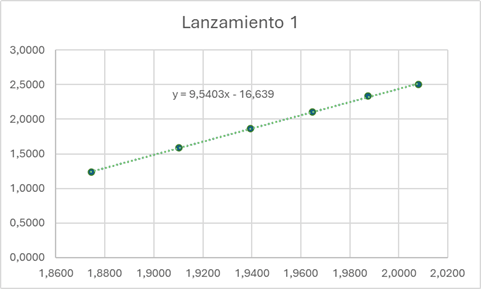
\includegraphics[width=0.45\textwidth]{docs/graficos/Grafico_1.png}
\caption{Gráfico de velocidad en función del tiempo para el lanzamiento 1.}
\label{fig:grafico1}
\end{figure}

\begin{figure}[H]
\centering
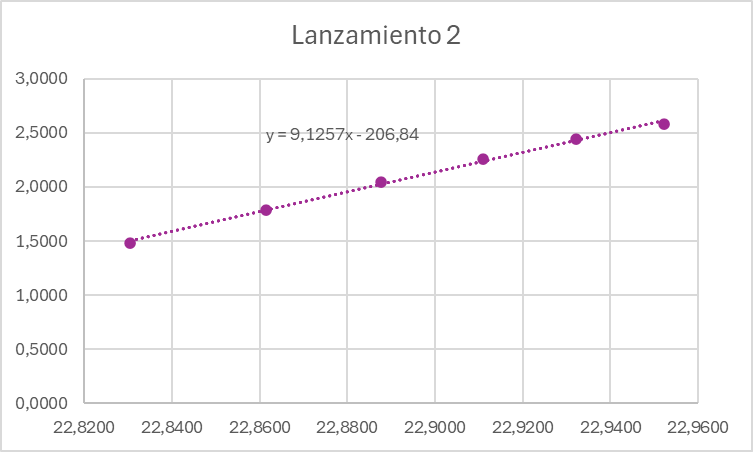
\includegraphics[width=0.45\textwidth]{docs/graficos/Grafico_2.png}
\caption{Gráfico de velocidad en función del tiempo para el lanzamiento 2.}
\label{fig:grafico2}
\end{figure}

\begin{figure}[H]
\centering
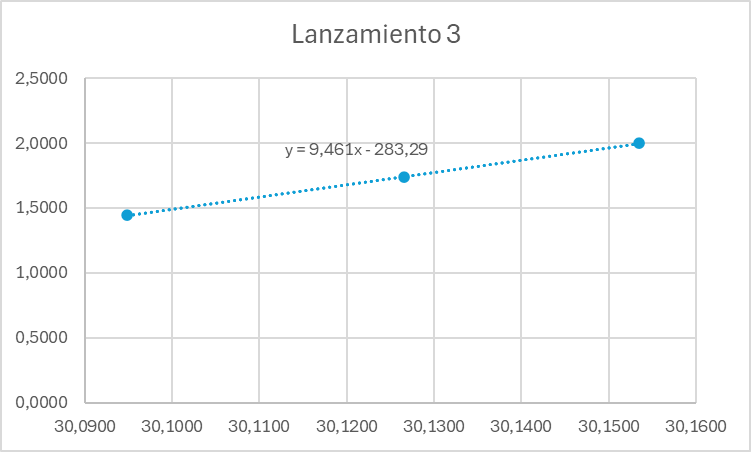
\includegraphics[width=0.45\textwidth]{docs/graficos/Grafico_3.png}
\caption{Gráfico de velocidad en función del tiempo para el lanzamiento 3.}
\label{fig:grafico3}
\end{figure}

En el tercer lanzamiento no se obtuvo la cantidad completa de intervalos temporales esperados, por lo que el conjunto de datos disponibles fue menor que en los otros lanzamientos. Esto implicó trabajar con menos puntos en la gráfica velocidad en función del tiempo, de modo que el ajuste lineal del lanzamiento 3 posee una menor robustez estadística y, por tanto, una mayor incertidumbre relativa en comparación con los lanzamientos 1 y 2.

A partir de los ajustes lineales de los Gráficos 1, 2 y 3, se obtuvieron las ecuaciones mostradas en la Tabla 6. Como establece la guía, la pendiente de cada recta representa la aceleración experimental del lanzamiento correspondiente.

\begin{table}[H]
\centering
\footnotesize
\begin{tabular}{ccc}
\toprule
Lanz. & Ajuste lineal & $g$ (m/s²) \\
\midrule
1 & $v = 9,5403 t - 16,639$ & 9,5403 \\
2 & $v = 9,1257 t - 206,84$ & 9,1257 \\
3 & $v = 9,4610 t - 283,29$ & 9,4610 \\
\bottomrule
\end{tabular}
\caption{Ajustes lineales del procedimiento 2.}
\end{table}

Usando las pendientes de la Tabla 6 como valores experimentales de $g$, y aplicando las ecuaciones (8), (9) y (10), se obtuvo el resumen estadístico mostrado en la Tabla 7.

\begin{table}[H]
\centering
\small
\begin{tabular}{cc}
\toprule
Magnitud & Valor \\
\midrule
Media $\bar{x}$ & 9,38 m/s² \\
Desviación estándar $s$ & 0,22 m/s² \\
Error estándar $d_x$ & 0,13 m/s² \\
\bottomrule
\end{tabular}
\caption{Resumen estadístico del procedimiento 2.}
\end{table}

Por lo tanto, el resultado final del procedimiento 2 se expresa como:
\begin{equation}
g_2 = (9,38 \pm 0,13) \text{ m/s²}
\end{equation}

% ======================== IV. ANÁLISIS DE RESULTADOS ========================
\section{Análisis de resultados}

En el primer procedimiento, basado en el uso de cronómetro, se obtuvo para la aceleración de gravedad un valor de $g=(14,61 \pm 1,62)\ \text{m/s}^2$. Sin embargo, este resultado no constituye una buena estimación de la aceleración de gravedad, ya que los valores obtenidos presentan una dispersión alta entre sí y varios de ellos se alejan considerablemente del valor teórico esperado, $9,8\ \text{m/s}^2$. Esto sugiere que el método manual estuvo fuertemente afectado por errores experimentales, especialmente por la medición del tiempo con cronómetro.

En cambio, en el segundo procedimiento, realizado con fotocelda, se obtuvo un valor de $g=(9,38 \pm 0,13)\ \text{m/s}^2$, mucho más cercano al valor teórico y con un error estándar notablemente menor. Esto indica que el procedimiento 2 entregó resultados más consistentes y confiables que el procedimiento 1.

Además, los gráficos de velocidad en función del tiempo obtenidos con la fotocelda muestran una tendencia lineal clara, lo que resulta consistente con el modelo cinemático de caída libre, en el cual la pendiente de la recta representa una aceleración aproximadamente constante. De esta forma, el comportamiento observado respalda la validez del procedimiento 2 como método experimental para estimar la aceleración de gravedad.

Cabe señalar que, en el tercer lanzamiento del procedimiento 2, no se registró la cantidad completa de intervalos esperados, por lo que se dispuso de un menor número de datos válidos. En consecuencia, el ajuste lineal de este lanzamiento presenta una mayor incertidumbre relativa que los lanzamientos 1 y 2. Sin embargo, esta limitación no afecta de manera importante la precisión general del método automatizado frente al método manual.

En términos generales, la comparación entre ambos procedimientos permite observar que el uso de instrumentación automática mejora significativamente la calidad de los resultados experimentales, especialmente cuando se trabaja con intervalos de tiempo muy pequeños.

% ======================== V. ANÁLISIS DE ERRORES ========================
\section{Análisis de errores}

La gran discrepancia observada en los resultados del procedimiento 1 puede atribuirse principalmente al tiempo de reacción humana al iniciar y detener el cronómetro. Dado que los tiempos de caída medidos fueron muy breves, inferiores a $0,7\ \text{s}$, un tiempo de reacción del orden de $0,2\ \text{s}$ introduce una incertidumbre porcentual muy alta, afectando significativamente el valor calculado de la aceleración de gravedad. A esto se suma la posible presencia de error de paralaje en la lectura de las alturas iniciales.

Por otro lado, el procedimiento 2 redujo considerablemente la influencia del error humano al automatizar la adquisición de datos mediante la fotocelda. La diferencia que aún se observa entre el valor experimental obtenido, $9,38\ \text{m/s}^2$, y el valor teórico esperado, $9,8\ \text{m/s}^2$, puede explicarse por la presencia de errores sistemáticos. Entre ellos, destaca la resistencia del aire, que no se considera en el modelo teórico ideal y que puede producir una aceleración efectiva ligeramente menor. Asimismo, pueden existir pequeñas desviaciones en la verticalidad de la regleta al atravesar el sensor, lo que también influye en la precisión de la medición.

% ======================== VI. CONCLUSIONES ========================
\section{Conclusiones}

El experimento permitió cumplir el objetivo principal de determinar experimentalmente la aceleración de la gravedad mediante dos metodologías distintas. Los resultados obtenidos permiten confirmar la hipótesis planteada: es posible estimar el valor de $g$ a partir del estudio del movimiento de caída libre, aunque la confiabilidad del resultado depende directamente de la técnica de medición utilizada.

A partir de la comparación entre ambos procedimientos, se concluye que el sistema automatizado de adquisición de datos mediante fotocelda es claramente superior al método manual con cronómetro, tanto en precisión como en exactitud, especialmente cuando se trabaja con intervalos de tiempo muy breves.

Finalmente, el análisis gráfico del procedimiento 2 permitió corroborar experimentalmente que, en una aproximación de caída libre ideal, la aceleración de un cuerpo se mantiene aproximadamente constante en el tiempo, en concordancia con el modelo teórico estudiado.

\end{multicols}

% ======================== REFERENCIAS ========================
% Referencias en una sola columna
\section*{Referencias}
\addcontentsline{toc}{section}{Referencias}

\noindent [1] Pontificia Universidad Católica de Chile, Instituto de Física. Laboratorio 1: Caída libre, FIS-1510L.

\end{document}
